\documentclass{article}
\usepackage[utf8]{inputenc}


\usepackage{amsmath}
\usepackage{amsfonts}
\usepackage{geometry}
\usepackage{booktabs}
\usepackage{graphicx}
\usepackage{listings}
\usepackage{xcolor}

% Define colors for listings
\definecolor{mygreen}{rgb}{0,0.6,0}
\definecolor{mygray}{rgb}{0.5,0.5,0.5}
\definecolor{mymauve}{rgb}{0.58,0,0.82}

% Configure listings package for MATLAB
\lstset{
    language=Matlab,
    basicstyle=\ttfamily\footnotesize,
    keywordstyle=\color{blue},
    commentstyle=\color{mygreen},
    stringstyle=\color{mymauve},
    numbers=left,
    numberstyle=\tiny\color{mygray},
    stepnumber=1,
    numbersep=5pt,
    backgroundcolor=\color{white},
    showspaces=false,
    showstringspaces=false,
    showtabs=false,
    frame=single,
    tabsize=2,
    captionpos=b,
    breaklines=true,
    breakatwhitespace=false,
    escapeinside={\%*}{*)}
}

\geometry{
 a4paper,
 total={170mm,257mm},
 left=20mm,
 top=20mm,
}
\usepackage{graphicx}
\usepackage{titling}

\title{Electromagnetism: Homework}
\author{Alessandro Crotti}
\date{Janueary 2025}

\usepackage{fancyhdr}
\fancypagestyle{plain}{%
    \fancyhf{}
    \fancyfoot[L]{\thedate}
    \fancyhead[L]{Electromagnetism}
    \fancyhead[R]{\theauthor}
}
\makeatletter
\def\@maketitle{%
  \newpage
  \null
  \vskip 1em%
  \begin{center}%
  \let \footnote \thanks
    {\LARGE \@title \par}%
    \vskip 1em%
  \end{center}%
  \par
  \vskip 1em}
\makeatother

\usepackage{lipsum}  
\usepackage{cmbright}

\begin{document}

\maketitle

\section{Exercise 1}
The following sections provide a comprehensive overview of various computational methods and their implementation for analyzing slab waveguides. Initially, we will explore the Fast Fourier Transform (FFT) Beam Propagation Method (BPM) tailored for slab waveguides. Subsequently, we will examine the application of the Finite Difference Scheme to the same problem, considering specific boundary conditions. The final two sections detail the implementation of the Finite Difference Method (FDM) in slab structures, with a particular focus on TE and TM modes.

\subsection{Point 1: FFT bpm slab}
We analyze the propagation of an optical field in a planar dielectric waveguide using the Beam Propagation Method (BPM) based on the Fast Fourier Transform (FFT) algorithm. The system consists of a symmetric slab waveguide with the following characteristics:
\begin{itemize}
    \item Core refractive index: $n_{co} = 1.495$
    \item Cladding refractive index: $n_{cl} = 1.3$
    \item Waveguide half-width: $a = 0.25\,\mu m$
    \item Operating wavelength: $\lambda = 1.5\,\mu m$
\end{itemize}
The propagation is governed by the paraxial wave equation (Fresnel equation):
\begin{equation}
    -j\frac{\partial\psi}{\partial z} + \frac{1}{2\kappa}\nabla_t^2\psi + \frac{\kappa}{2}\left(\frac{n^2(x,z)}{n_0^2} - 1\right)\psi = 0
\end{equation}
where $\psi$ is the optical field, $\kappa$ is the reference wavenumber, and $n(x,z)$ is the refractive index profile.

\subsubsection{Numerical Implementation}
The simulation employs a split-step approach:
\begin{enumerate}
    \item A propagation step in the Fourier domain accounting for diffraction
    \item A phase correction step in the spatial domain accounting for the refractive index variations
\end{enumerate}

The propagation is analyzed over a distance of $50\,\mu m$ with $5000$ iterations, ensuring accurate modeling of both the diffractive and refractive effects. The computational window extends to $\pm 6.4\,\mu m$ in the transverse direction, sampled with $256$ points.

\subsubsection{Initial Condition}
The initial field distribution corresponds to the fundamental TE$_0$ mode of the symmetric slab waveguide, pre-calculated and loaded from external data. This represents a physically meaningful starting point as it corresponds to the natural guided mode of the structure.

\subsubsection{Expected Behavior}
The simulation should demonstrate:
\begin{itemize}
    \item Stable propagation of the guided mode
    \item Confinement of light within the core region
    \item Conservation of field energy throughout propagation
\end{itemize}

This analysis provides insights into the wave-guiding properties of the structure and validates the effectiveness of the FFT-BPM implementation for modeling optical waveguide phenomena.

We present the results of two distinct cases: with and without the thin lens law operator. The simulation was performed using the FFT-BPM method over a propagation distance of $50 \,\mu m$.

\begin{figure}[h]
\centering
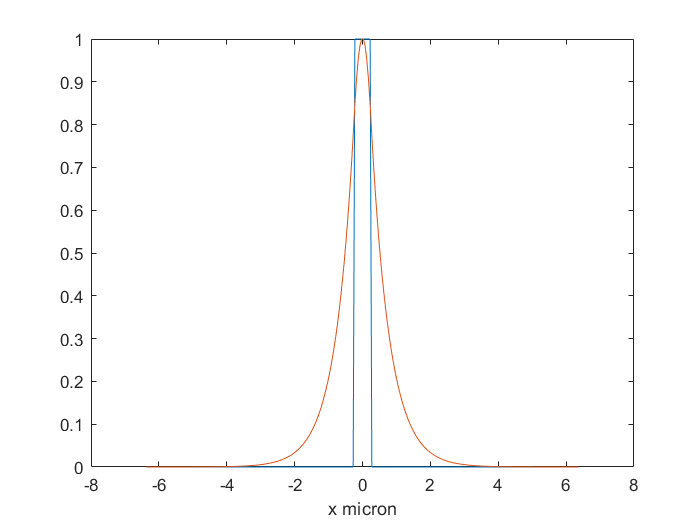
\includegraphics[width=0.45\textwidth]{es1/1/front_view_without_thin_lens_law_op.png}
\caption{Initial conditions showing the fundamental TE$_0$ mode (red line) and the normalized refractive index profile (blue line).}
\label{fig:initial}
\end{figure}

\subsubsection{Case 1: Without Thin Lens Law Operator}
\begin{figure}[h]
\centering
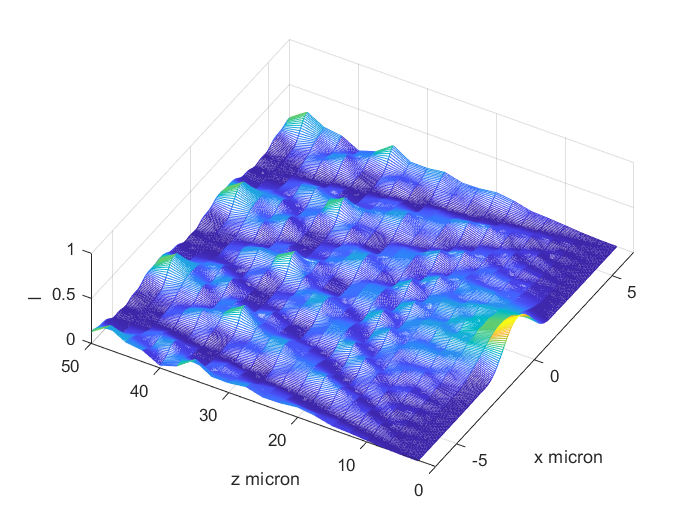
\includegraphics[width=0.45\textwidth]{es1/1/3D_without_thin_lens_law_op.png}
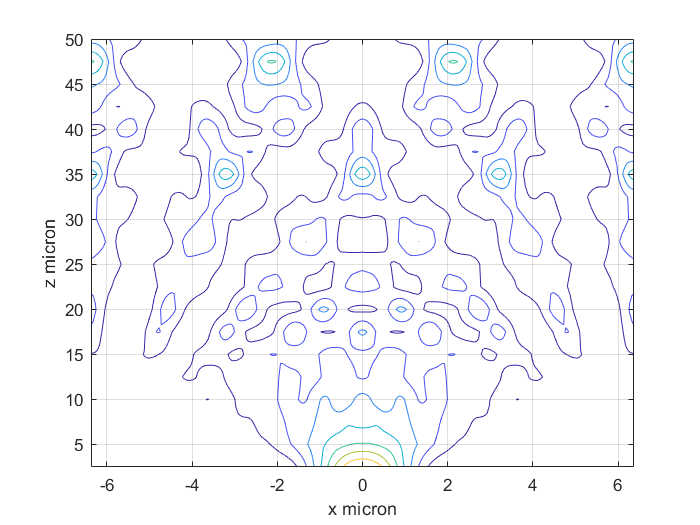
\includegraphics[width=0.45\textwidth]{es1/1/3d_UPVIEW_view_without_thin_lens_law_op.png}
\caption{Field propagation without the thin lens law operator}
\label{fig:no_lens}
\end{figure}

When the thin lens law operator is disabled, we observe in Fig. \ref{fig:no_lens} that the field maintains its initial Gaussian-like shape but gradually diffracts. The energy spreads in the transverse direction as the beam propagates and no confinement effect from the waveguide structure is visible. The simulation shows pure diffraction behavior without the guiding effect of the refractive index variation.

\subsubsection{Case 2: With Thin Lens Law Operator}
\begin{figure}[h]
\centering
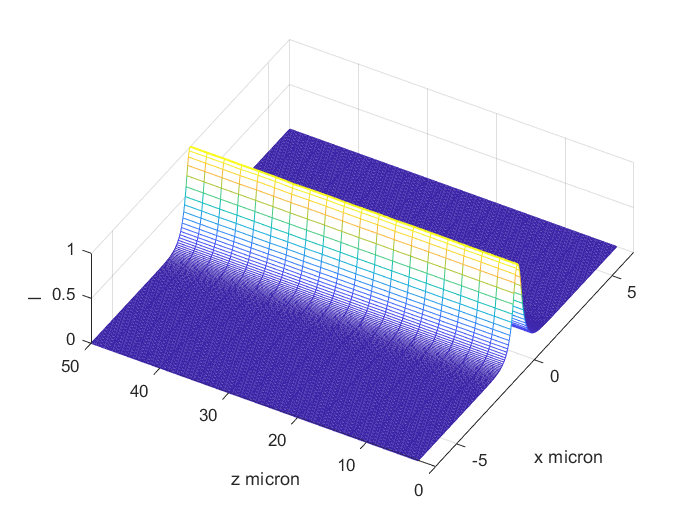
\includegraphics[width=0.45\textwidth]{es1/1/3D.png}
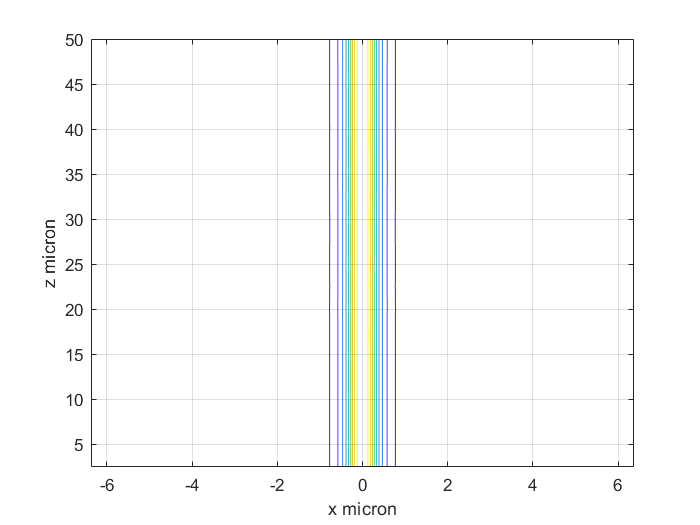
\includegraphics[width=0.45\textwidth]{es1/1/3D_UPVIEW.png}
\caption{Field propagation with the thin lens law operator}
\label{fig:with_lens}
\end{figure}

With the thin lens law operator enabled, the field remains strongly confined within the core region, as we can see in Fig. \ref{fig:with_lens}. The mode profile maintains its shape throughout propagation and the waveguiding effect is clearly visible, demonstrating proper modal confinement. The simulation accurately represents the physical behavior of a guided mode in a dielectric waveguide.

\subsubsection{Comparison and Discussion}
The comparison between the two cases clearly demonstrates the crucial role of the thin lens law operator in modeling waveguide behavior. Without the operator, the simulation only accounts for diffraction effects, missing the essential physics of waveguiding. With the operator, the simulation correctly models both diffraction and the guiding effect of the refractive index profile. The thin lens law operator is essential for accurately representing the phase modifications induced by the refractive index variations. The results with the operator enabled match the expected behavior of a guided mode in a dielectric waveguide.

This analysis confirms that the thin lens law operator is fundamental for accurate modeling of optical waveguide propagation using the FFT-BPM method.






\subsection{Point 2: FD bpm slab}
\subsubsection{FD-BPM Implementation Results}

We analyze the results of the Finite Difference Beam Propagation Method (FD-BPM) implementation in a planar dielectric waveguide. The system consists of a symmetric slab waveguide with core refractive index $n_{co} = 1.495$ and cladding refractive index $n_{cl} = 1.3$. The waveguide half-width is $a = 0.25\,\mu m$, and the operating wavelength is $\lambda = 1.5\,\mu m$. The simulation extends over a propagation distance of $50\, \mu m$ with $5000$ iterations. 

In the code implementation, we completed several crucial parts:
\begin{itemize}
\item The Fresnel equation term for refractive index changes: 
   $(guide^2 - n_0^2)/(2n_0^2)$, representing the normalized index variation.
\item The transparent boundary conditions for the left border, implementing the energy outflow condition with appropriate phase matching.
\item The thin lens law operator: $exp(-j \cdot xk \cdot guide \cdot deltaz)$, accounting for the refractive index-induced phase changes.

\end{itemize}


\begin{figure}[h]
\centering
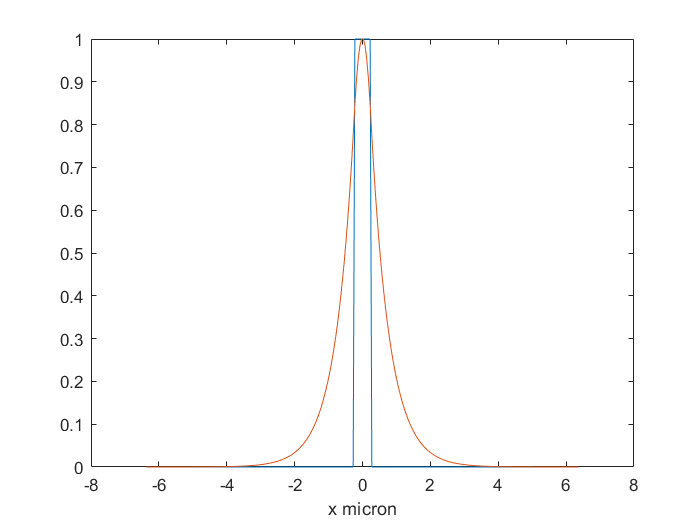
\includegraphics[width=0.45\textwidth]{es1/2/FRONT_VIEW_TRASPARENT.png}
\caption{Initial field distribution (red line) and normalized refractive index profile (blue line) for the FD-BPM simulation.}
\label{fig:initial_fd}
\end{figure}


\begin{figure}[h]
\centering
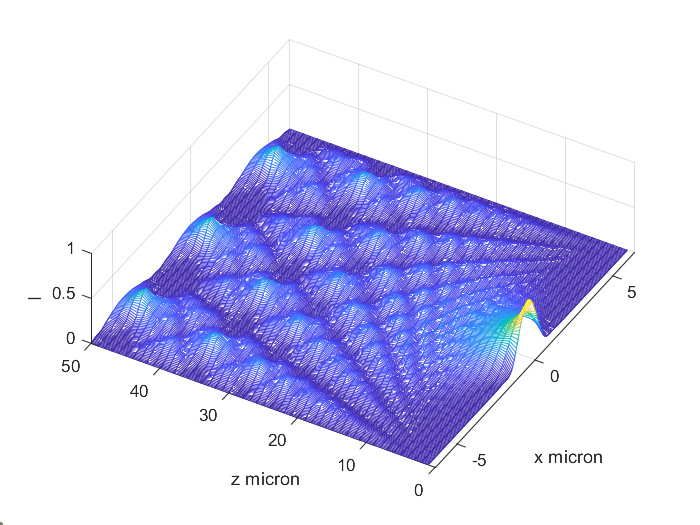
\includegraphics[width=0.45\textwidth]{es1/2/3D_NEUMANN_WITHOUT.png}
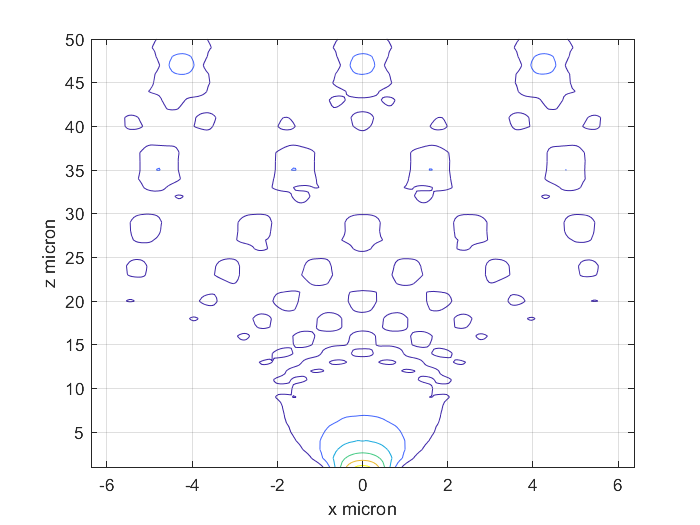
\includegraphics[width=0.45\textwidth]{es1/2/3D_UPVIEW_NEUMANN_WITHOUT.png}
\caption{Field propagation with Neumann boundary conditions, without thin lens law operator}
\label{fig:neumann_no_lens}
\end{figure}

\begin{figure}[h]
\centering
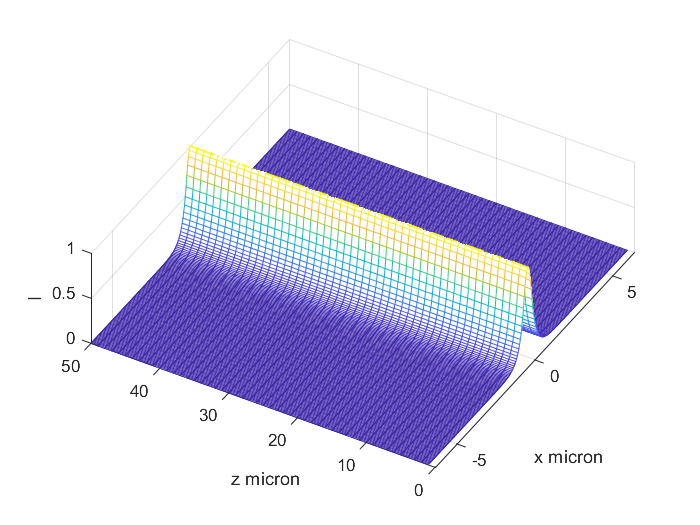
\includegraphics[width=0.45\textwidth]{es1/2/3D_NEUMANN.png}
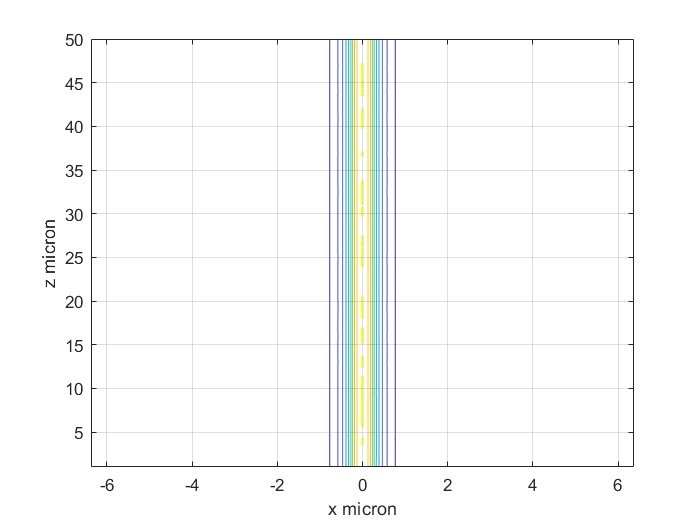
\includegraphics[width=0.45\textwidth]{es1/2/3D_UPVIEW_NEUMANN.png}
\caption{Field propagation with Neumann boundary conditions, with thin lens law operator}
\label{fig:neumann_with_lens}
\end{figure}



\begin{figure}[h]
\centering
    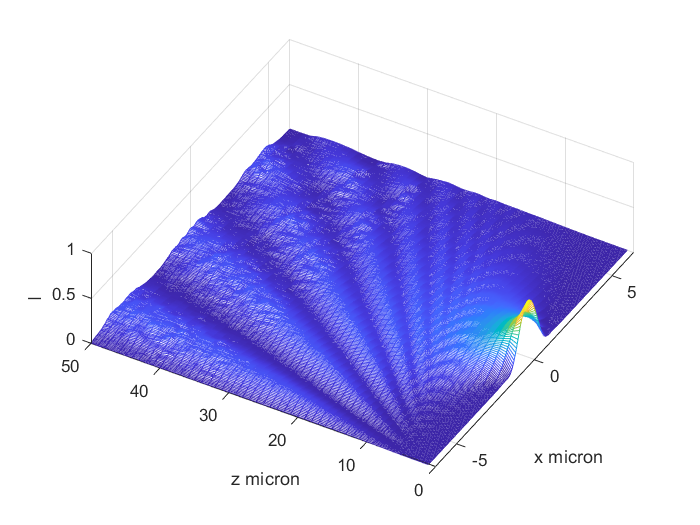
\includegraphics[width=0.45\textwidth]{es1/2/3D_TRASPARENT_WITHOUT.png}
    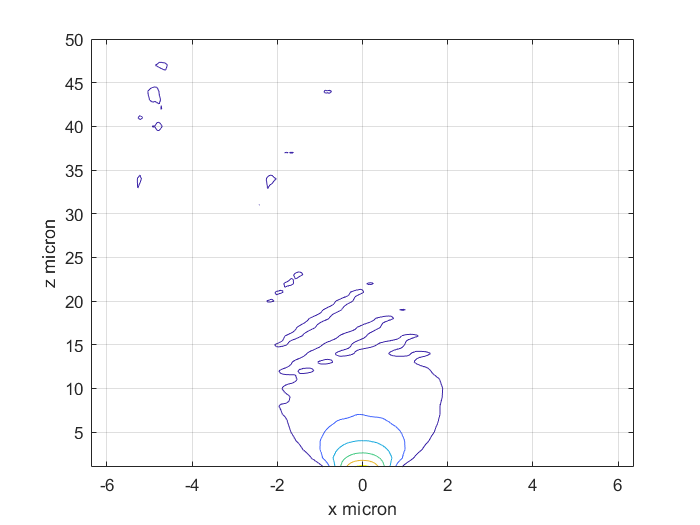
\includegraphics[width=0.45\textwidth]{es1/2/3D_UPVIEW_TRASPARENT_WITHOUT.png}
\caption{Field propagation with transparent boundary conditions, without thin lens law operator}
\label{fig:tbc_no_lens}
\end{figure}

\begin{figure}[h]
\centering
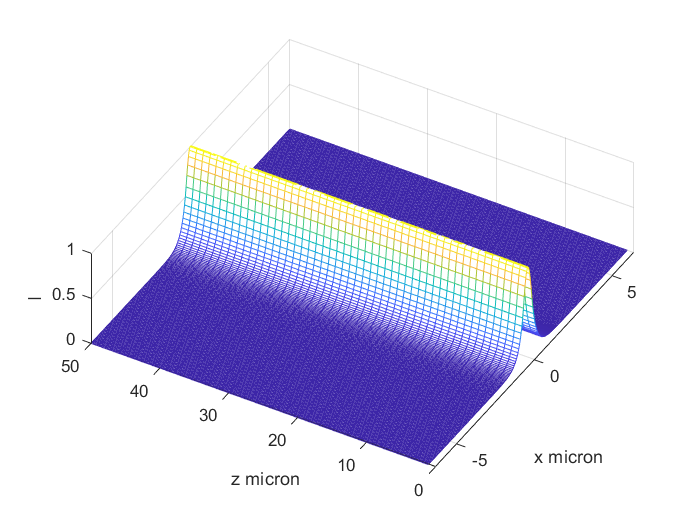
\includegraphics[width=0.45\textwidth]{es1/2/3D_TRASPARENT.png}
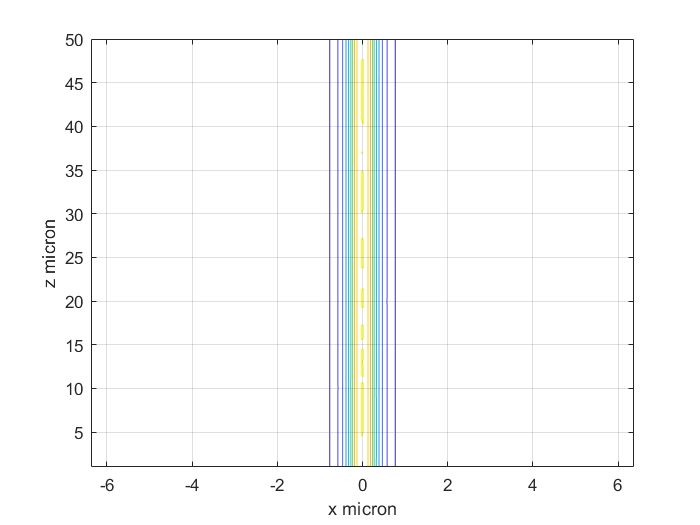
\includegraphics[width=0.45\textwidth]{es1/2/3D_UPVIEW_TRASPARENT.png}
\caption{Field propagation with transparent boundary conditions, with thin lens law operator}
\label{fig:tbc_with_lens}
\end{figure}





\subsubsection{Analysis and Discussion}

The simulation results demonstrate the fundamental differences between boundary conditions and the effect of the thin lens law operator in waveguide propagation modeling.

The simulation results clearly demonstrate the fundamental differences between Neumann and Transparent Boundary Conditions in waveguide modeling. Looking at the contour plots and 3D visualizations, we can observe several key distinctions:

In the case of Neumann Boundary Conditions Fig. \ref{fig:neumann_with_lens}, the field shows perfect confinement within the computational window. This is an artificial effect caused by the zero-derivative constraint at the boundaries ($\partial\psi/\partial x = 0$). While this might seem advantageous for guided modes, it creates an unrealistic perfect reflection at the boundaries, essentially turning the computational window edges into perfect mirrors. This behavior is particularly evident in the contour plot, where the field maintains a strict confinement pattern throughout the propagation distance.

In contrast, the Transparent Boundary Conditions (TBC) implementation provides a more physically realistic behavior. The TBC allows the radiative components of the field to naturally exit the computational window, preventing artificial reflections. This is achieved through the exponential field behavior assumption at the boundaries:
\begin{equation}
\psi = \psi_0\exp(-j\kappa_xx)
\end{equation}
where $\kappa_x$ is dynamically calculated during propagation. The contour plot for TBC shows a more natural field evolution, where any radiative components can smoothly exit the computational domain without creating interference patterns from artificial reflections.

The 3D visualization further emphasizes these differences. With Neumann conditions, we observe a sharp cutoff at the boundaries, while the TBC implementation shows a more gradual field decay. This natural decay is particularly important for accurately modeling:
\begin{itemize}
    \item Radiative losses in waveguides
    \item Mode coupling phenomena
    \item Leaky modes and radiation modes
\end{itemize}

The superiority of TBC becomes evident in long-distance propagation simulations, where accumulated artificial reflections from Neumann boundaries would significantly distort the field distribution. TBC maintains the physical integrity of the simulation while efficiently handling the computational domain boundaries.





The Neumann boundary conditions Fig. \ref{fig:neumann_with_lens} - \ref{fig:neumann_no_lens}, implemented by forcing zero field derivatives at the boundaries, show significant limitations in our simulation. These conditions create artificial reflections at the computational window edges, particularly visible in the 3D propagation view. The reflections interfere with the propagating field, creating unrealistic patterns in the field distribution.

The Transparent Boundary Conditions, implemented through the exponential field behavior assumption at the boundaries, demonstrate superior performance. By allowing radiation to exit the computational window while preventing inward propagation, these conditions provide a more physically accurate representation of the waveguide behavior. The implementation involves careful calculation of the transverse wavenumber κx and appropriate phase matching at the boundaries.

\subsubsection{Effect of Thin Lens Law Operator}
The thin lens law operator plays a crucial role in modeling the waveguiding effect. Without this operator, we observe pure diffraction behavior, where the field energy spreads across the computational window without any guiding effect. This is clearly visible in the diffraction patterns of the field intensity Fig. \ref{fig:neumann_no_lens}-\ref{fig:tbc_no_lens}.

With the operator enabled, the simulation accurately captures the waveguiding phenomenon. The field remains confined within the core region, maintaining its modal profile throughout propagation. This confinement results from the proper implementation of the phase corrections induced by the refractive index variations.

\subsubsection{Conclusions}
Our FD-BPM implementation successfully demonstrates the interplay between boundary conditions and the thin lens law operator in waveguide modeling. The combination of Transparent Boundary Conditions with the thin lens law operator provides the most physically accurate results, correctly modeling both the guided modes and radiating fields. The implementation shows how proper handling of boundary conditions and refractive index variations is crucial for accurate optical waveguide simulation.

The completed code sections ensure energy conservation, proper phase matching at boundaries, and accurate modeling of the waveguiding effect, making this implementation a reliable tool for studying optical waveguide phenomena.





\subsection{Point 3: FDM TE}

In the study of optical waveguides, determining the supported modes is essential for understanding light propagation characteristics. This section elucidates the physical principles implemented in a Finite Difference Method (FDM) based modal solver for Transverse Electric (TE) family modes. The solver specifically addresses the eigenvalue problem associated with the wave equation in a dielectric waveguide structure.

\subsubsection{Waveguide Structure and Governing Equations}

Consider a planar dielectric waveguide composed of a core with refractive index $n_{\text{co}}$ and a cladding with refractive index $n_{\text{cl}}$. The waveguiding occurs in the transverse $x$-direction with the propagation along the $z$-axis. For TE modes, the electric field has only a $y$-component, $E_y(x)$, and satisfies the Helmholtz equation:

\begin{equation}
\frac{d^2 E_y}{dx^2} + \left( k_0^2 n^2(x) - \beta^2 \right) E_y = 0,
\end{equation}

where:
\begin{itemize}
    \item $k_0 = \dfrac{2\pi}{\lambda}$ is the wave number in vacuum,
    \item $n(x)$ is the refractive index profile,
    \item $\beta$ is the propagation constant.
\end{itemize}

\subsubsection{Finite Difference Discretization}

The transverse domain is discretized into $N_p$ points with uniform spacing $\Delta x$. The second derivative in the Helmholtz equation is approximated using the finite difference scheme:

\begin{equation}
\frac{d^2 E_y}{dx^2} \approx \frac{E_{i+1} - 2E_i + E_{i-1}}{(\Delta x)^2}.
\end{equation}
Substituting this into the Helmholtz equation leads to a matrix eigenvalue problem of the form:

\begin{equation}
\mathbf{A} \mathbf{E} = \beta^2 \mathbf{E},
\end{equation}
where $\mathbf{A}$ is a tridiagonal matrix with elements:

\begin{align}
A_{i,i} &= \frac{2}{(\Delta x)^2} - k_0^2 n^2(x_i), \\
A_{i,i+1} = A_{i+1,i} &= -\frac{1}{(\Delta x)^2}.
\end{align}

In the provided MATLAB code, the matrix $\mathbf{A}$ is constructed with the following steps:

The principal diagonal elements of $\mathbf{A}$ incorporate both the finite difference approximation and the refractive index profile:

\begin{equation}
A(i,i) = k_0^2 n^2(x_i) - \frac{2}{(\Delta x)^2}.
\end{equation}
This accounts for the term $k_0^2 n^2(x)$ from the Helmholtz equation and the finite difference approximation of the second derivative.

The upper and lower diagonals of $\mathbf{A}$ are set as:

\begin{equation}
A(i, i+1) = A(i+1, i) = \frac{1}{(\Delta x)^2},
\end{equation}
representing the coupling between adjacent points due to the second derivative.

After constructing the matrix $\mathbf{A}$, the eigenvalue problem is solved using MATLAB's \texttt{eig} function:

\begin{equation}
\mathbf{A} \mathbf{V} = \mathbf{V} \mathbf{D},
\end{equation}
where $\mathbf{V}$ contains the eigenvectors (mode profiles) and $\mathbf{D}$ is a diagonal matrix with eigenvalues $\beta^2$.

\subsubsection{Post-Processing and Mode Selection}

To ensure that only physically meaningful guided modes are considered, the following criteria are applied:

Since $\beta^2$ represents the square of the propagation constant, only real and positive eigenvalues correspond to propagating modes:

\begin{equation}
\text{If } \Re(\beta^2) > 0, \text{ then } \beta = \sqrt{\beta^2} \text{ is real and positive.}
\end{equation}
This eliminates spurious solutions that may arise from numerical discretization.

The effective refractive index $n_{\text{eff}}$ is defined as:

\begin{equation}
n_{\text{eff}} = \frac{\beta}{k_0}.
\end{equation}
For a mode to be guided, its effective index must lie between the refractive indices of the core and the cladding:

\begin{equation}
n_{\text{cl}} \leq n_{\text{eff}} \leq n_{\text{co}}.
\end{equation}
This condition ensures that the mode is confined within the core and decays exponentially in the cladding.


For each valid mode, the corresponding eigenvector is normalized and plotted against the transverse coordinate $x$. The mode profile $E_y(x)$ illustrates the spatial distribution of the electric field within the waveguide, confirming confinement in the core region.


Hai ragione, ecco come dovrebbe essere strutturato il testo con l'inclusione appropriata delle immagini in LaTeX:

\subsubsection{Results and Discussion}

The numerical analysis of the waveguide modes for different wavelengths revealed significant characteristics of light propagation. The FDM solver was executed for three distinct wavelengths: $\lambda = 0.7\,\mu m$, $\lambda = 1.0\,\mu m$, and $\lambda = 1.5\,\mu m$, yielding the following results:

For $\lambda = 0.7\,\mu m$, two guided modes were identified:
\begin{itemize}
\item First mode: $n_{\text{eff}} = 1.4381$ Fig.\ref{fig:TE_mode_07_1}
\item Second mode: $n_{\text{eff}} = 1.3025$ Fig.\ref{fig:TE_mode_07_2}
\end{itemize}

\begin{figure}[h]
\centering
\includegraphics[width=0.8\textwidth]{es1/3/lambda_0.7.png}
\caption{First TE mode at $\lambda = 0.7\,\mu m$ with $n_{\text{eff}} = 1.4381$}
\label{fig:TE_mode_07_1}
\end{figure}

\begin{figure}[h]
\centering
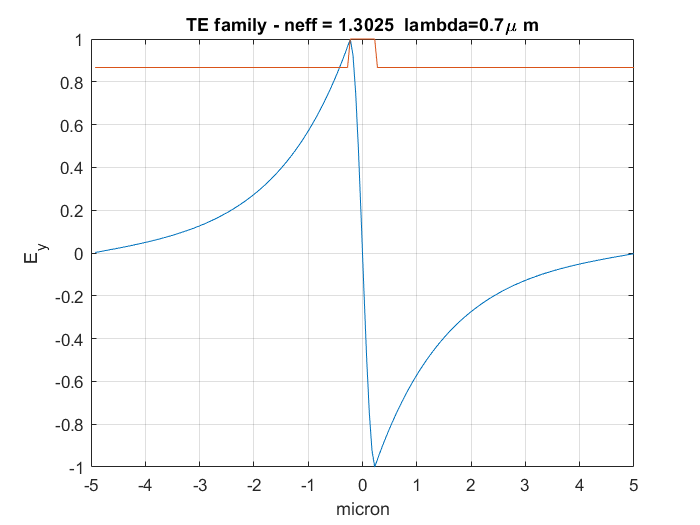
\includegraphics[width=0.8\textwidth]{es1/3/lambda_0.7_2.png}
\caption{Second TE mode at $\lambda = 0.7\,\mu m$ with $n_{\text{eff}} = 1.3025$}
\label{fig:TE_mode_07_2}
\end{figure}

The presence of two modes at this wavelength is attributed to the shorter wavelength allowing multiple solutions to satisfy the wave equation within the waveguide's physical constraints. As shown in Figures \ref{fig:TE_mode_07_1} and \ref{fig:TE_mode_07_2}, the first mode exhibits strong confinement in the core, while the second mode shows a broader field distribution but remains within the guidance condition $n_{\text{cl}} < n_{\text{eff}} < n_{\text{co}}$.

At $\lambda = 1.0\,\mu m$, the analysis revealed a single guided mode with $n_{\text{eff}} = 1.409$:

\begin{figure}[h]
\centering
\includegraphics[width=0.8\textwidth]{es1/3/lambda_1.png}
\caption{TE mode at $\lambda = 1.0\,\mu m$ with $n_{\text{eff}} = 1.409$}
\label{fig:TE_mode_10}
\end{figure}

The mode profile in Fig.\ref{fig:TE_mode_10} demonstrates excellent confinement within the core region, with the electric field amplitude decaying appropriately in the cladding regions.

For $\lambda = 1.5\,\mu m$, one guided mode was observed with $n_{\text{eff}} = 1.3734$:

\begin{figure}[h]
\centering
\includegraphics[width=0.8\textwidth]{es1/3/lambda_1.5.png}
\caption{TE mode at $\lambda = 1.5\,\mu m$ with $n_{\text{eff}} = 1.3734$}
\label{fig:TE_mode_15}
\end{figure}

The increased wavelength results in a more extended field distribution compared to the $\lambda = 1.0\,\mu m$ case, while maintaining proper waveguiding characteristics as you can see in Fig.\ref{fig:TE_mode_15}.

The modal analysis demonstrates the wavelength-dependent nature of waveguide operation:
\begin{itemize}
\item Shorter wavelengths ($\lambda = 0.7\,\mu m$) support multiple modes due to increased spatial frequency components fitting within the waveguide dimensions
\item Longer wavelengths ($\lambda = 1.0\,\mu m$ and $\lambda = 1.5\,\mu m$) exhibit single-mode operation, ideal for applications requiring controlled light propagation
\item All identified modes satisfy the fundamental waveguiding condition, with effective indices properly bounded between core and cladding indices
\end{itemize}

These results align with theoretical predictions and provide valuable insights for waveguide design in practical applications. The field distributions, as shown in the figures, validate the numerical implementation and demonstrate proper mode confinement across all wavelengths studied.












\subsection{Point 4: FDM TM}

In optical waveguide analysis, the study of Transverse Magnetic (TM) modes complements the TE mode analysis. This section presents the implementation of a Finite Difference Method (FDM) based modal solver for TM family modes, where the magnetic field has only a $y$-component.

\subsubsection{Waveguide Structure and Governing Equations}

For TM modes in a planar dielectric waveguide, the magnetic field component $H_y(x)$ satisfies the modified Helmholtz equation:

\begin{equation}
\frac{d}{dx}\left(\frac{1}{n^2(x)}\frac{dH_y}{dx}\right) + \left(k_0^2 - \frac{\beta^2}{n^2(x)}\right)H_y = 0,
\end{equation}

where:
\begin{itemize}
\item $k_0 = \dfrac{2\pi}{\lambda}$ is the wave number in vacuum,
\item $n(x)$ is the refractive index profile,
\item $\beta$ is the propagation constant.
\end{itemize}

\subsubsection{Finite Difference Discretization}

The TM wave equation differs from the TE case due to the presence of $\frac{1}{n^2(x)}$ terms. The finite difference approximation must account for these variations in the refractive index. The discretized form becomes:

\begin{equation}
\frac{2}{n^2(x_i)\Delta x^2}\left[k_r H_{i+1} + k_l H_{i-1} - (1-r_r-r_l)H_i\right] + k_0^2 H_i = \beta^2 H_i,
\end{equation}

where:
\begin{align}
k_r &= \frac{n^2(x_{i+1})}{n^2(x_i) + n^2(x_{i+1})}, \\
k_l &= \frac{n^2(x_{i-1})}{n^2(x_i) + n^2(x_{i-1})}, \\
r_r &= \frac{n^2(x_{i+1}) - n^2(x_i)}{n^2(x_{i+1}) + n^2(x_i)}, \\
r_l &= \frac{n^2(x_{i-1}) - n^2(x_i)}{n^2(x_{i-1}) + n^2(x_i)}.
\end{align}

\subsubsection{Matrix Formulation}

The discretized equation leads to an eigenvalue problem:

\begin{equation}
\mathbf{A} \mathbf{H} = \beta^2 \mathbf{H},
\end{equation}

where the matrix elements are:

\begin{align}
A_{i,i} &= -\frac{2(1-r_r-r_l)}{\Delta x^2} + k_0^2 n^2(x_i), \\
A_{i,i+1} &= \frac{2k_r}{\Delta x^2}, \\
A_{i+1,i} &= \frac{2k_l}{\Delta x^2}.
\end{align}

\subsubsection{Results and Discussion}

The TM modal solver was executed for three wavelengths: $\lambda = 0.7\,\mu m$, $\lambda = 1.0\,\mu m$, and $\lambda = 1.5\,\mu m$. The results demonstrate the following characteristics:

For $\lambda = 0.7\,\mu m$, similar to the TE case, two guided modes were identified:
\begin{itemize}
\item First mode: $n_{\text{eff}} = 1.4381$ Fig.\ref{fig:TM_mode_07_1}
\item Second mode: $n_{\text{eff}} = 1.3025$ Fig.\ref{fig:TM_mode_07_2}
\end{itemize}

\begin{figure}[h]
\centering
\includegraphics[width=0.8\textwidth]{es1/4/lambda_0.7.png}
\caption{First TM mode at $\lambda = 0.7\,\mu m$}
\label{fig:TM_mode_07_1}
\end{figure}

\begin{figure}[h]
\centering
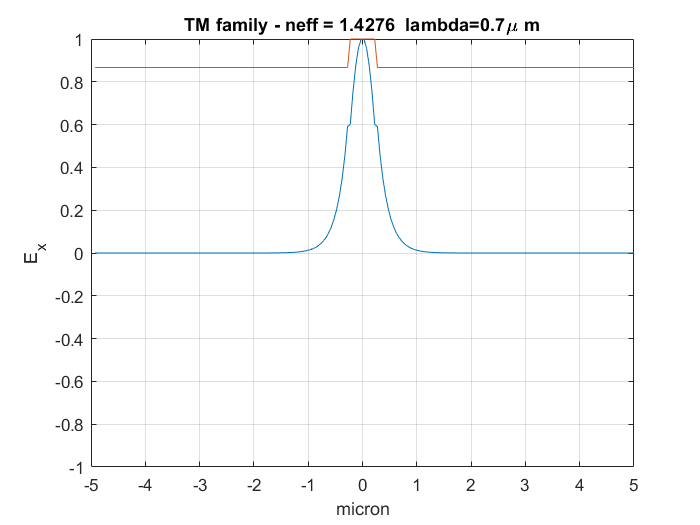
\includegraphics[width=0.8\textwidth]{es1/4/lambda_0.7_1.png}
\caption{Second TM mode at $\lambda = 0.7\,\mu m$}
\label{fig:TM_mode_07_2}
\end{figure}

For $\lambda = 1.0\,\mu m$ and $\lambda = 1.5\,\mu m$ as you can see in Fig.\ref{fig:TM_mode_10} and Fig.\ref{fig:TM_mode_15} respectively, single-mode operation was observed:

\begin{figure}[h]
\centering
\includegraphics[width=0.8\textwidth]{es1/4/lambda_1.png}
\caption{TM mode at $\lambda = 1.0\,\mu m$}
\label{fig:TM_mode_10}
\end{figure}

\begin{figure}[h]
\centering
\includegraphics[width=0.8\textwidth]{es1/4/lambda_1.5.png}
\caption{TM mode at $\lambda = 1.5\,\mu m$}
\label{fig:TM_mode_15}
\end{figure}

The key differences between TM and TE modes include:
\begin{itemize}
\item TM modes show slightly different field distributions due to the boundary condition discontinuities at the core-cladding interface
\item The effective indices for TM modes are generally lower than their TE counterparts due to weaker confinement
\item The modal profiles exhibit characteristic asymmetry at the core-cladding boundaries due to the $\frac{1}{n^2(x)}$ term in the wave equation
\end{itemize}



\section{Exercise 2}
On this exercise we create a waveguide with the CST program. The walls of the rectangular waveguide are composed by PEC and filled with vacuum. We simulate the propagation from port1 to port2 using the time domain solver. We get the following results as you can see in the table and in Fig. \ref{fig:tablees2}. 
\subsection{vacuum}
\subsubsection{MODE 1}
\begin{itemize}
    \item mode: $\text{TE}_{10}$
    \item Cutoff frequency: $5 \, GHz$
    \item degeneracy: No
\end{itemize}

\subsubsection{MODE 2}
\begin{itemize}
    \item mode: $\text{TE}_{20}$
    \item Cutoff frequency: $10 \, Ghz$
    \item degeneracy: No
\end{itemize}

\subsubsection{MODE 3}
\begin{itemize}
    \item mode: $\text{TE}_{01}$
    \item Cutoff frequency: $12.5 \, GHz$
    \item degeneracy: NO
\end{itemize}

\subsubsection{MODE 4}
\begin{itemize}
    \item mode: $\text{TE}_{11}$
    \item Cutoff frequency: $13.5 \, GHz$
    \item degeneracy: YES
\end{itemize}

\begin{figure}[h]
\centering
\includegraphics[width=0.8\textwidth]{es2/Screenshot 2025-01-31 170224.png}
\caption{Table of exercise 2 with the mode and cut-off frequency reported}
\label{fig:tablees2}
\end{figure}

\subsection{teflon}
In the case of teflon as inner material, we change from time domain solver to frequency domain solver setting the working frequency of $10.7\,GHz$ as the single frequency of the simulation. After the costruction of the mesh, we can run the simulation obtaining a similar result but with a lower cutoff frequency because the relative electric permettivity is higher than vacuum and this lowers the cutoff frequency. Furthermore, every mode can propagate in this configuration.
$$\text{cutoff frequency}_{\text{TE}_{10}} = 3.5\,GHz$$
$$\text{cutoff frequency}_{\text{TE}_{20}} = 6.9\,GHz$$
$$\text{cutoff frequency}_{\text{TE}_{01}} = 8.6\,GHz$$
$$\text{cutoff frequency}_{\text{TE}_{11}} = 9.3\,GHz$$






\section{Exercise 3}
At Port 1, we can see the propagation of the fundamental mode. The program was able to understand that this solution is of TEM type, without z components for both the electrical field and the magnetic field. There is no cutoff frequency and the wave is able to propagate at any low frequency. The lines of force of the electrical field are radial because, we know from the theory that they must be normal to any PEC surface.

The magnetic field must form loops, and these loops are enclosing electrical current density because we have a linear conductor. We have a transverse geometry which is no longer simply connected. This is compatible with Maxwell's equations.

The calculation of the wave impedance is the ratio between the components of the electric and magnetic fields transverse with respect to the direction of calculation, and they are completely transverse. We have seen from the theory that the fundamental mode of a structure which is no longer simply connected has the same features as the uniform plane wave in the corresponding material.

The wave impedance, which is the value of the intrinsic impedance, is the value of the impedance of Teflon $\frac{1}{\sqrt{\epsilon \mu}}$.

We also have the line impedance, which is the ratio between the phasor of voltage and the phasor of current. These are complex numbers, so line impedance could be complex. However, in a structure where we have PEC and an ideal dielectric inner material, the line impedance is purely real. Consequently, the power carried by voltage and current waves is purely active.

Line impedance and wave impedance would have higher values if the inner material were vacuum, but in this case, we have Teflon which has a higher permittivity, and this lowers the impedances. If we want to change the value of the line impedance, we should change the dimensions of the coaxial cable.

Concerning the second modal solution, the type is transverse electric and we have a cutoff frequency of $3.39871\,GHz$. In any case, the lines of force must be normal to the PEC conductor and the PEC shield, and we have an azimuthal dependence (transverse electromagnetic solution is independent of the azimuthal coordinates).

The corresponding magnetic field should have lines of force that form closed loops in the transverse plane, with both radial and azimuthal components. Unlike the fundamental TEM mode, this TE mode has a longitudinal component of the magnetic field, while the electric field remains entirely transverse. The magnetic field lines form a more complex pattern compared to the fundamental mode, with variations in both the radial and azimuthal directions. This modal structure results in higher losses and greater dispersion compared to the fundamental TEM mode, which is why coaxial cables are typically operated below the cutoff frequency of this second mode to maintain single-mode operation.

With these results, we can identify the unimodal region under the cutoff frequency of the second modal solution $3.39871\,GHz$ where only the first mode is allowed to propagate.

In mode 1, we have an undistorted propagation from port 1 to port 2. Increasing the frequency, we have a shrinking of the spatial period. In the second mode, we can see the presence of the cutoff frequency. The electric and magnetic field is unable to propagate until the cutoff frequency; then at $4\,GHz$, we can see propagation with the same effect of shrinking of the spatial period at higher frequencies.

Looking at the surface current, we can find interesting features. The surface current is longitudinal in both the inner and outer conductors. The wave of current is made by surface current flowing on the inner conductor, and we also have inner current on the inner part of the shield. 
we can see the same effect of shrinking of the spatial period at higher frequencies and the presence of cutoff frequency for the second mode.






\section{Exercise 4}
\subsection{Half-wavelength dipole in transmitting mode}

\subsubsection{a) Time-domain solver simulation (FDTD)}
Once the set up is ready and the simulation has been done in the frequency range 400-800 MHz, we can see the results. The simulation has been performed using the Time-domain solver (FDTD) which allows us to analyze the antenna's behavior across the specified frequency range.

\subsubsection{b) Radiation solid and polar diagrams}
First of all, we explore the farfield region at $600\,MHz$ and here we can see the radiation solid Fig. \ref{fig:radiation solid}. The dipole, aligned with the z axis, produces a radiation pattern, the solid representing the modulus of the pointing vector on a sphere. It displays how the power density is distributed on a sphere. 

What we see in the figures should be the Fraunhofer region. Then, we have local plane wave approximation and this is in dB scale; in this way, we have a value proportional to the power and not to the magnetic or electric field.

In Linear scale, we can see the real 3D function, and the axial symmetry for the radiated energy is clearly visible. The function depends on $\theta$ angle. This is the angle between the z axis and the general point.

In order to check if we have a value close to the square of the sin function for what concerns the behavior of the plane containing the antenna, we can see the intersection of the solid with the specific plane which usually contains the antenna (e.g.$ z-y, z-x$). The result is evaluated for each value of the $\theta$ angle, the absolute value of Farfield directivity which is proportional to the pointing vector for $\phi = 90°$ Fig. \ref{fig:dir_phi_90}. A similar point of view can be seen for the Gain Fig. \ref{fig:gain_phi_90}-\ref{fig:gain_theta_90}.

We can also change the intersection of the radiation solid and the plane, and $\theta = 90°$ is now fixed Fig.\ref{fig:dir_theta_90}. Then we are orthogonal to the z axis and we have a circle, thus the antenna is omnidirectional but only in this plane.
We have verified that the half wavelength dipole working at $600 \, MHz$ is radiating as we expected from the theory. We have the radiation solid independent from the phi azimuthal angle and it is completely omnidirectional on the plane orthogonal to the z axis; this concerns the directivity.

We can now take a look at some parameters such as the directivity which is the maximum value of the radiation solid and it is equal to $1.682$ which is close to the analytical value.
Another interesting value is the Gain, which is related to the directivity. It is in practice the ratio between the power that would be needed for an isotropic antenna and the feeding power. Being the antenna made by PEC and immersed in vacuum, we don't have losses in any point of the numerical box. In practice, the gain and the directivity must give us the same value.

\subsubsection{c) Input impedance behavior}
Being the situation ideal, the radiation efficiency is equal to $1.000$. The total efficiency, which is not present in our theory, comes out from the presence of the impedance of the generator $75 \Omega$. This is due to the not perfect matching between the generator and the antenna. The antenna is seen as a load described by an impedance value. We want to maximize the transfer of active power from the generator to the antenna which transforms the input energy into radiating energy. The maximum transfer of power happens when the value of the impedance of the generator is equal to the complex conjugate of the load. The impedance of the generator is $75 \,\Omega$ which is close to the value of the half dipole antenna's impedance. Then, we are close to the maximum transfer of active power. 

We can see the real part of the impedance for each frequency simulated in Fig. \ref{fig:real_impedence} (red line). We can see the Impedance at the working frequency of the antenna which is bigger than the generator's impedance set at the beginning. But, looking at the imaginary part \ref{fig:immaginary_impedence} (red line) we can see that it is not close to zero. Then looking at the value of frequency where the imaginary part goes to zero we have a closer value in the real part. But this new frequency, having fixed dimensions of the antenna and having a not negligible diameter, is not feasible. Furthermore, having a gap between the two wires, we have a capacity factor added in parallel to the electrical circuit. 

In order to raise the radiation efficiency and total efficiency we have to lower the length of the antenna about $0.08\%$. Then we get:
$$\text{rad. efficiency = }1.000$$
$$\text{tot. efficiency = }0.9993$$
We can see the new impedance in Fig. \ref{fig:real_impedence} (yellow line) for the real part and \ref{fig:immaginary_impedence} (yellow line) for the imaginary part. The radiation solid changes as we can see in Fig. \ref{fig:radiation solid_1}.





\begin{figure}[h]
\centering
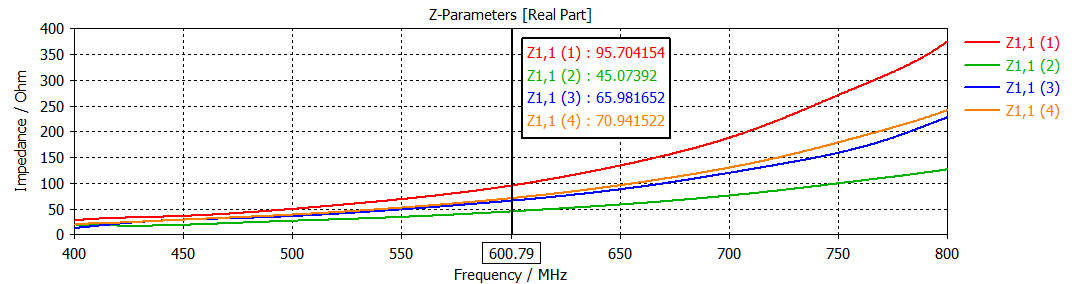
\includegraphics[width=0.8\textwidth]{es4/Z1,1_2.png}
\caption{Real part of impedence respect to different lengths of the antenna}
\label{fig:real_impedence}
\end{figure}

\begin{figure}[h]
\centering
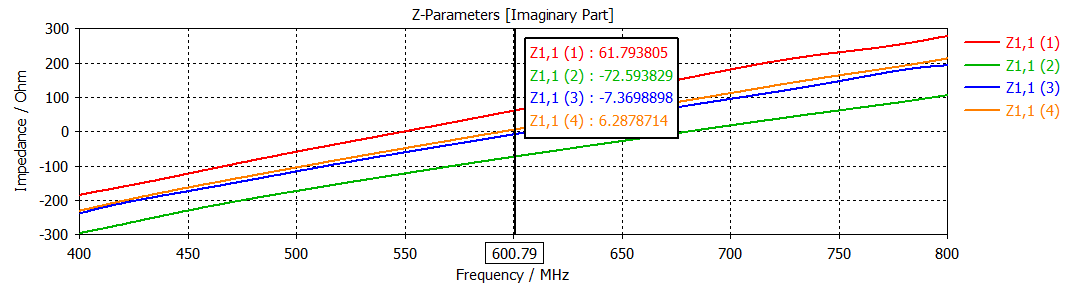
\includegraphics[width=0.8\textwidth]{es4/Z1,1_3.png}
\caption{Immaginary part of impedence respect to different lengths of the antenna}
\label{fig:immaginary_impedence}
\end{figure}

\begin{figure}[h]
\centering
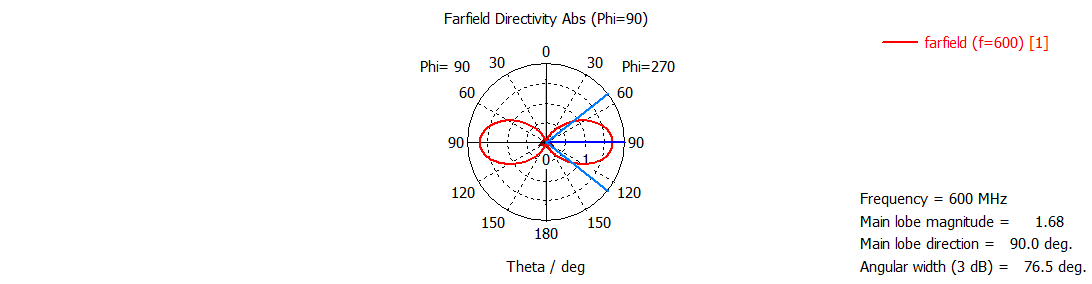
\includegraphics[width=0.8\textwidth]{es4/dir_phi_90.png}
\caption{Directivity at $\phi$ setted to $90°$}
\label{fig:dir_phi_90}
\end{figure}

\begin{figure}[h]
\centering
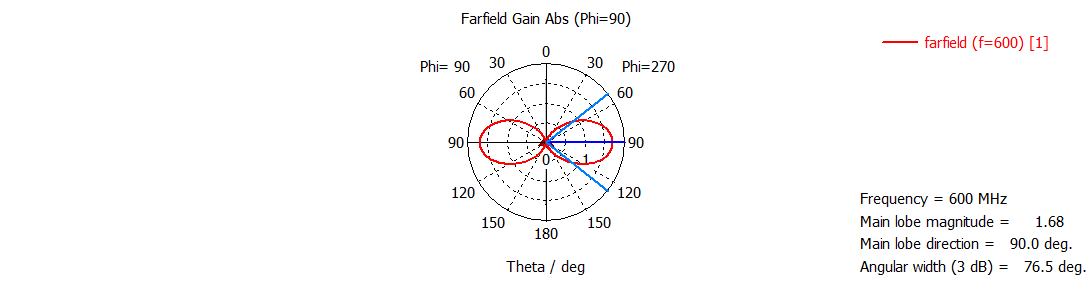
\includegraphics[width=0.8\textwidth]{es4/gain_phi_90.png}
\caption{Gain at $\phi$ setted to $90°$}
\label{fig:gain_phi_90}
\end{figure}

\begin{figure}[h]
\centering
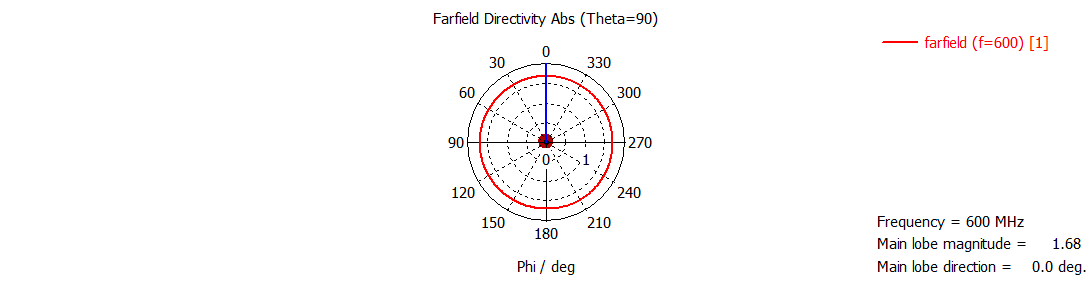
\includegraphics[width=0.8\textwidth]{es4/dir_theta_90.png}
\caption{Directivity at $\theta$ setted to $90°$}
\label{fig:dir_theta_90}
\end{figure}

\begin{figure}[h]
\centering
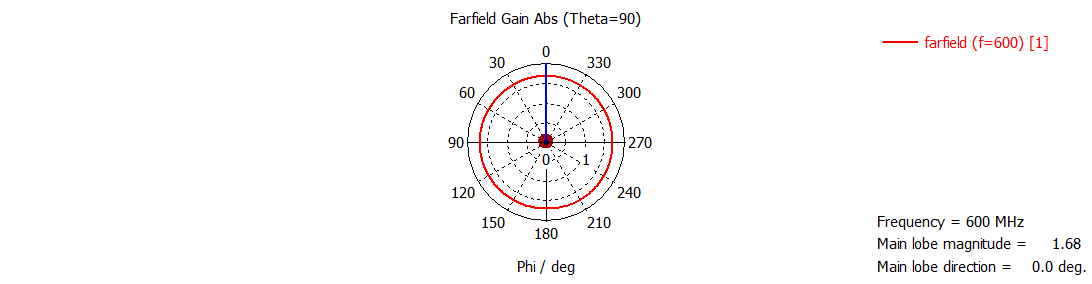
\includegraphics[width=0.8\textwidth]{es4/gain_theta_90.png}
\caption{Gain at $\theta$ setted to $90°$}
\label{fig:gain_theta_90}
\end{figure}


\begin{figure}[h]
\centering
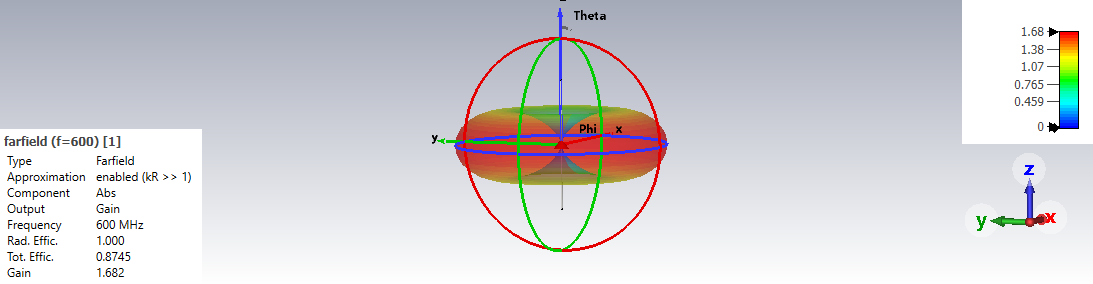
\includegraphics[width=0.8\textwidth]{es4/rad_sol_1.png}
\caption{Radiation solid at the begging configuration}
\label{fig:radiation solid}
\end{figure}

\begin{figure}[h]
\centering
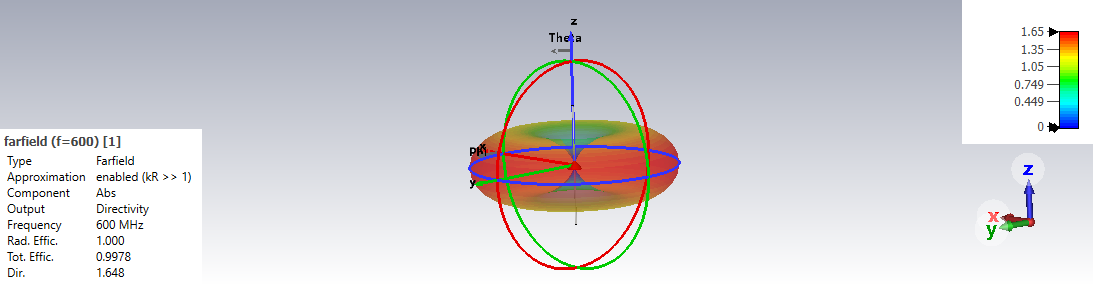
\includegraphics[width=0.8\textwidth]{es4/sol_rad_2.png}
\caption{Radiation solid with the modified length of the antenna}
\label{fig:radiation solid_1}
\end{figure}





\subsection{Half-wavelength dipole in receiving mode}

\subsubsection{d) Time-domain solver simulation with plane-wave excitation}
When analyzing the half-wavelength dipole in receiving mode, we need to consider the antenna's behavior when intercepting electromagnetic waves rather than generating them. The simulation using plane-wave excitation allows us to understand the antenna's receiving characteristics.

In receiving mode, the antenna is excited by an incident plane wave with linear polarization parallel to the $z-\text{axis}$ and propagating along the $x-\text{axis}$ with an amplitude of $10 V/m$. This configuration is crucial because the receiving efficiency is maximum when the polarization of the incident wave matches the antenna's orientation. 

Looking at the open voltage in this configuration (Fig. \ref{fig:open_voltage_1}), we can observe its behavior across the frequency range. The maximum value occurs at the resonant frequency, where the antenna's length matches half the wavelength. This is expected as the antenna is most efficient at its design frequency.

\begin{figure}[h]
\centering
% Place for first open voltage plot
\caption{Open voltage with plane wave propagating along x-axis and E-field along z-axis}
\label{fig:open_voltage_1}
\end{figure}

The reciprocity theorem ensures that the radiation pattern in receiving mode mirrors that of the transmitting mode, making the half-wavelength dipole equally effective in both configurations when properly oriented with respect to the polarization of the electromagnetic wave.

\subsubsection{e) Voltage probe measurements with rotating polarization}
The voltage probe placed in the gap allows us to measure the induced voltage at the center frequency. For the second case, we rotate the plane wave configuration to have a $10 V/m$ amplitude along the $x-\text{axis}$ and propagation along the $y-\text{axis}$. The open voltage in this new configuration (Fig. \ref{fig:open_voltage_2}) shows a different behavior due to the changed orientation of the incident field relative to the antenna axis.

\begin{figure}[h]
\centering
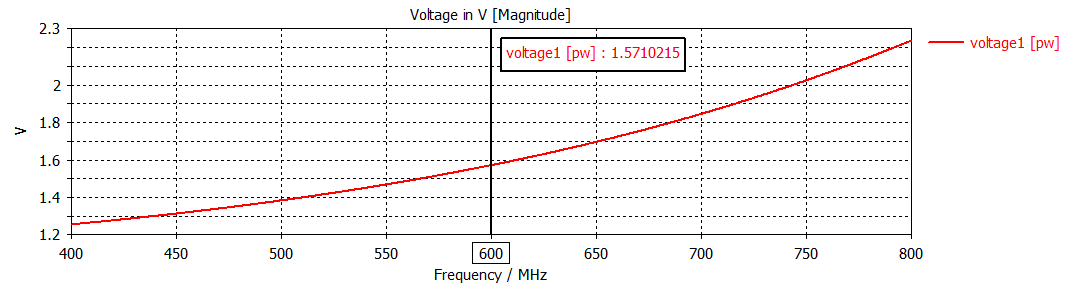
\includegraphics[width=0.8\textwidth]{es4/open voltage d.png}
\caption{Open voltage with plane wave propagating along y-axis and E-field along x-axis}
\label{fig:open_voltage_2}
\end{figure}

By rotating the direction of polarization of the impinging plane wave from 0° to 360°, we can observe how the received voltage varies with the polarization angle. This follows the cosine law:

$$ V_{received} = V_{max} \cos(\alpha) $$

where $\alpha$ is the angle between the antenna axis and the polarization direction of the incident wave.

\begin{figure}[h]
\centering
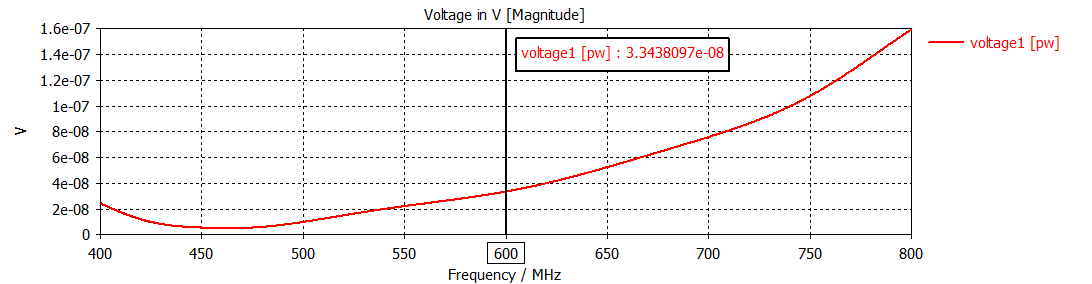
\includegraphics[width=0.8\textwidth]{es4/open voltage c.png}
\caption{Received voltage vs. polarization angle}
\label{fig:voltage_vs_angle}
\end{figure}

This behavior demonstrates the antenna's polarization sensitivity, which is a fundamental characteristic of linear antennas. Maximum reception occurs when the incident wave's electric field is parallel to the antenna axis ($\alpha = 0°$), while no voltage is induced when the polarization is perpendicular to the antenna ($\alpha = 90°$). The comparison between the two open voltage measurements clearly shows how the antenna's response changes with different incident wave configurations.

\end{document}


